% Author: Izaak Neutelings (October 2020)
\documentclass[border=3pt,tikz]{standalone}
\usepackage{physics}
\usepackage{siunitx}
\usepackage{tikz}
\usetikzlibrary{calc}
\usetikzlibrary{angles,quotes} % for pic
\usetikzlibrary{arrows.meta}
\usetikzlibrary{bending} % for arrow head angle
\tikzset{>=latex} % for LaTeX arrow head
\usetikzlibrary{patterns}

\colorlet{xcol}{blue!70!black}
\colorlet{vcol}{green!60!black}
\colorlet{myred}{red!65!black}
\colorlet{mypurple}{blue!60!red!80}
\colorlet{acol}{red!50!blue!80!black!80}
\tikzstyle{rvec}=[->,xcol,very thick,line cap=round]
\tikzstyle{vvec}=[->,vcol,very thick,line cap=round]
\tikzstyle{myarr}=[{Latex[length=3,width=3]}-,xcol]
\tikzstyle{myarr2}=[{Latex[length=2,width=3]}-{Latex[length=2,width=3]}]
\tikzstyle{force}=[->,myred,very thick,line cap=round]
\tikzstyle{Fproj}=[force,myred!40]
\tikzstyle{myarr}=[-{Latex[length=4,width=3]}]
\tikzstyle{myarr2}=[{Latex[length=4,width=3]}-{Latex[length=3,width=3]}]
\tikzstyle{CM}=[red!40!black,fill=red!80!black!80]
\tikzstyle{mass}=[line width=0.6,draw=red!30!black, %rounded corners=1,
                  top color=red!40!black!30,bottom color=red!40!black!10,shading angle=30]
\tikzstyle{ground}=[preaction={fill,top color=black!10,bottom color=black!5,shading angle=20},
                    fill,pattern=north east lines,draw=none,minimum width=0.3,minimum height=0.6]
\tikzstyle{metal}=[fill,top color=black!40,bottom color=black!20,shading angle=10]
\def\tick#1#2{\draw[thick] (#1) ++ (#2:0.1) --++ (#2-180:0.2)}
\tikzstyle{ladder}=[brown!40!black,fill=brown!70!black,thin,line cap=round]
\tikzstyle{limb}=[thick,line cap=round]


\def\LL{4.7}  % ladder length
\def\LR{0.06} % ladder radius
\def\r{0.04}  % pulley small radius
\tikzset{
  pics/Tin/.style={
    code={
      \def\R{0.12}
      \draw[pic actions,line width=0.6,#1,fill=white] % ,thick
        (0,0) circle (\R) (-135:.75*\R) -- (45:.75*\R) (-45:.75*\R) -- (135:.75*\R);
  }},
  pics/Tout/.style={
    code={
      \def\R{0.12}
      \draw[pic actions,line width=0.6,#1,fill=white] (0,0) circle (\R);
      \fill[pic actions,#1] (0,0) circle (0.3*\R);
  }},
  pics/ladder/.style={
    code={
      \coordinate (L1) at (0,\LR+0.01);
      \draw[ladder] (L1)++(#1-90:\LR) arc(#1-90:#1-270:\LR) --++ (#1:{\LL-\LR/cos(\ang)}) arc(90+#1:#1-90:\LR) -- cycle;
      \coordinate (L2) at ($(L1)+(#1:\LL/2)$);
      \coordinate (L3) at ($(L1)+(#1:{\LL-\LR/cos(\ang)})$);
  }},
  pics/groundwall/.style={
    code={
      \draw[ground] ({-0.26*\W},0) rectangle ({1.18*\W},-\D);
      \draw[thick] ({-0.26*\W},0) -- ({1.18*\W},0);
      \foreach \i[evaluate={\by=\i*\bh}]  in {0,...,\N}{ %[evaluate={\bh=\H/\N;\by=\i*\bh}] in {0,...,\N}{
      \draw[red!40!black,fill=red!40!black!40,rounded corners=0.8]
        ({\W},\by) rectangle++ (1.2*\D,\bh);
      \begin{scope}
        \clip ({\W+0.01},\by+0.01) rectangle++ (1.2*\D-0.02,\bh-0.02);
        \foreach \j in {0,...,\Nd}{
          \fill[red!40!black] ({\W+(1+rand)*0.6*\D},{\by+(1+rand)*\bh/2}) circle(0.002); % random dots
        }
      \end{scope}
    }
  }},
  pics/Tin/.default=mypurple,
  pics/Tout/.default=mypurple,
  pics/ladder/.default=45,
}

\begin{document}


% LADDER
\def\ang{50} % angle diagonal
\def\H{\LL*sin(\ang)} % ladder height
\def\W{\LL*cos(\ang)} % ladder width
\def\R{sqrt(\W^2+\H^2)/2} % block half-diagonal
\def\D{0.25}   % ground depth
\def\F{0.95}   % force
\def\Ff{0.85}  % force friction
\def\N{31}     % number of bricks
\def\Nd{30}    % number of dots per brick
\def\bh{0.125} % brick height
\begin{tikzpicture}
  \message{Ladder^^J}
  \coordinate (O) at (0,0);
  \coordinate (M) at (\ang:\LL/2);
  \coordinate (T) at (\ang:\LL);
  \coordinate (R) at ({\W},0);
  
  % GROUND + WALL
  \pic at (O) {groundwall};
  \draw[myarr2,thick] (-0.3*\F,{0.85*\H}) node[left,scale=0.8] {$y$} |-++ (0.65*\F,-0.65*\F) node[below,scale=0.8] {$x$};
  \draw[myarr,thick] (0.38*\F,{0.9*\H}) arc(100:10:0.35*\F) node[right=1,below=-1,scale=0.7] {$+$};
  
  % LADDER
  \pic[scale=1] at (O) {ladder={\ang}};
  \draw[CM] (L2) circle(0.9*\LR);
  \draw[force] (L1) --++ (\Ff,0) node[above right=-3] {$\vb{F}_\mathrm{f}$};
  \draw[force] (L1) --++ (0,\F) node[above=-2] {$\vb{F}_\mathrm{N}$};
  \draw[force] (L2) --++ (0,-\F) coordinate (FG) node[above right=0] {$M\vb{g}$};
  \draw[force] (L3) --++ (-\Ff,0) coordinate (FW) node[left=-3] {$\vb{F}_\mathrm{W}$};
  \draw[dashed] (L3) --++ (\ang:0.15*\LL) coordinate (T');
  \draw pic[->,"$\theta$"scale=0.9,draw,angle radius=12,angle eccentricity=1.4] {angle=R--O--T};
  \draw pic[<-,"$\dfrac{\pi}{2}-\theta$"{scale=0.8,above right=-5},draw,angle radius=9,angle eccentricity=1.5] {angle=FG--M--T};
  \draw pic[-{>[flex=1]},"$\pi-\theta$"{scale=0.8,above left=-5},draw,angle radius=9,angle eccentricity=1.4] {angle=T'--L3--FW};
\end{tikzpicture}


% LADDER + person
\begin{tikzpicture}
  \message{Ladder + person^^J}
  \def\h{1.2} % human height
  \coordinate (O) at (0,0);
  \coordinate (T) at (\ang:\LL);
  \coordinate (R) at ({\W},0);
  \coordinate (S) at ($(\ang:0.28*\LL)+(0,1.4*\LR)$);
  
  % GROUND + WALL
  \pic at (O) {groundwall};
  
  % PERSON
  \draw[thick] (S)++(0,\h) circle(0.22) coordinate (H);
  \draw[thick] (H)++(-90:0.22) coordinate (N) to[out=-91,in=92]++ (0,-0.35*\h) coordinate (P);
  \draw[limb] (N)++(-95:0.03) to[out=-120,in=-85]++ (-0.31*\h,0.22*\h); % right arm
  \draw[limb] (N)++(-85:0.03) to[out=-60,in=105]++ (0.19*\h,-0.35*\h);  % left arm
  \draw[limb] (S)++(\ang:0.06*\LL) to[out=85,in=-70,looseness=1.4] (P); % left leg
  \draw[limb] (S) to[out=85,in=-80] (P); % right leg
  
  % LADDER
  \pic[scale=1] at (O) {ladder={\ang}};
  \draw[CM] (L2) circle(0.9*\LR);
  \draw[force] (L1) --++ (\Ff,0) node[above=3,right=-3] {$\vb{F}_\mathrm{f}$};
  \draw[force] (L1) --++ (0,\F) node[left=2,above=-2] {$\vb{F}_\mathrm{N}$};
  \draw[force] (L2) --++ (0,-\F) node[above right=0] {$M\vb{g}$};
  \draw[force] (L3) --++ (-\Ff,0) node[left=-3] {$\vb{F}_\mathrm{W}$};
  \draw[force] (S)++(\ang:0.03*\LL) coordinate (SM) --++ (0,-0.58*\F) node[below right=-4] {$m\vb{g}$};
  \draw[rvec] (L1) -- (SM) node[midway,above=2] {$\vb{r}$};
  \draw pic[->,"$\theta$"scale=0.9,draw,angle radius=12,angle eccentricity=1.4] {angle=R--O--T};
  
\end{tikzpicture}


% LADDER + person
\begin{tikzpicture}
  \message{Ladder + person, shifted CM^^J}
  \def\h{1.2} % human height
  \coordinate (O) at (0,0);
  \coordinate (T) at (\ang:\LL);
  \coordinate (R) at ({\W},0);
  \coordinate (S) at ($(\ang:0.28*\LL)+(0,1.4*\LR)$);
  
  % GROUND + WALL
  \pic at (O) {groundwall};
  
  % PERSON
  \draw[thick] (S)++(0,\h) circle(0.22) coordinate (H);
  \draw[thick] (H)++(-90:0.22) coordinate (N) to[out=-91,in=92]++ (0,-0.35*\h) coordinate (P);
  \draw[limb] (N)++(-95:0.03) to[out=-120,in=-85]++ (-0.31*\h,0.22*\h); % right arm
  \draw[limb] (N)++(-85:0.03) to[out=-60,in=105]++ (0.19*\h,-0.35*\h);  % left arm
  \draw[limb] (S)++(\ang:0.06*\LL) to[out=85,in=-70,looseness=1.4] (P); % left leg
  \draw[limb] (S) to[out=85,in=-80] (P); % right leg
  
  % LADDER
  \pic[scale=1] at (O) {ladder={\ang}};
  \draw[CM] (L2)++(\ang-180:0.1*\LL) circle(0.9*\LR) coordinate (CM);
  \draw[force] (L1) --++ (\Ff,0) node[above right=-3] {$\vb{F}_\mathrm{f}$};
  \draw[force] (L1) --++ (0,\F) node[left=2,above=-2] {$\vb{F}_\mathrm{N}$};
  \draw[force] (CM) --++ (0,-\F) node[above right=0,scale=0.94] {$(m+M)\vb{g}$};
  \draw[force] (L3) --++ (-\Ff,0) node[left=-3] {$\vb{F}_\mathrm{W}$};
  %\draw[force] (S)++(\ang:0.03*\LL) coordinate (SM) --++ (0,-0.45*\F) node[below right=-4] {$m\vb{g}$};
  \draw[rvec] (L1) -- (CM) node[midway,above left=-2] {$\vb{r}$};
  \draw pic[->,"$\theta$"scale=0.9,draw,angle radius=12,angle eccentricity=1.4] {angle=R--O--T};
  
\end{tikzpicture}


% LADDER - tan
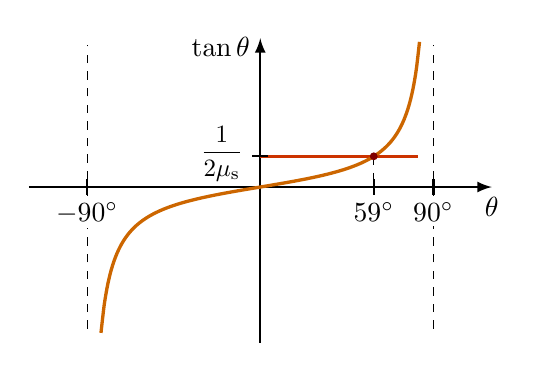
\begin{tikzpicture}
  \message{Plot numerical solution^^J}
  \def\xmax{2.8}
  \def\ymax{1.8}
  \def\A{0.13*\ymax}   % yscale
  \def\p{0.5*pi*\xmax} % xscale (in units of pi)
  \def\B{59/180}       % mu_s = 0.3
  \coordinate (O) at (0,0);
  \coordinate (B) at (\B*\p,{\A/2/0.3}); % mu_s = 0.3
  \coordinate (Bx) at (\B*\p,0);
  \coordinate (By) at (0,{\A/2/0.3});
  \draw[->,thick] (0,-1.1*\ymax) -- (0,1.05*\ymax) node[below=3,left] {$\tan\theta$};
  \draw[->,thick] (-1.05*\xmax,0) -- (1.05*\xmax,0) node[below] {$\theta$};
  \draw[dashed] (-\p/2,-\ymax) -- (-\p/2,\ymax);
  \draw[dashed] (\p/2,-\ymax) -- (\p/2,\ymax);
  \draw[line width=1.0,orange!50!red!80!black] (By) -- (B) --++ (0.2*\xmax,0);
  \draw[dashed] (B) -- (Bx);
  \tick{-\p/2,0}{90} node[below=0.7,scale=1,fill=white,inner sep=1.6] {$-\SI{90}{\degree}$}; %{$-\dfrac{\pi}{2}$};
  \tick{ \p/2,0}{90} node[below=0.7,scale=1,fill=white,inner sep=1.6] {$\SI{90}{\degree}$}; %{$\dfrac{\pi}{2}$};
  \tick{Bx}{90} node[below=-1,scale=1] {$\SI{59}{\degree}$};
  \tick{By}{0} node[above=1,left=0,scale=0.9] {$\dfrac{1}{2\mu_\mathrm{s}}$};
  \draw[very thick,orange!80!black,samples=100,smooth,variable=\t,domain=-0.46*\p:0.46*\p]
    plot(\t,{\A*tan(\t*180/(\p))});
  \fill[red!50!black] (B) circle(0.05);
\end{tikzpicture}

% LADDER - plot
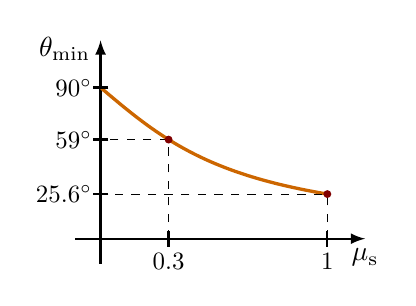
\begin{tikzpicture}
  \message{Minimum angle vs. mu_s^^J}
  \def\xmax{3.2}
  \def\ymax{2.4}
  \def\A{0.8*\ymax}   % yscale
  \def\k{0.9*\xmax}   % xscale
  \def\B{59/90*\A}    % mu_s = 0.3
  \def\C{26.57/90*\A} % mu_s = 1
  \coordinate (O) at (0,0);
  \coordinate (B) at (0.3*\k,\B);
  \coordinate (Bx) at (0.3*\k,0);
  \coordinate (By) at (0,\B);
  \coordinate (C) at (\k,\C);
  \coordinate (Cx) at (\k,0);
  \coordinate (Cy) at (0,\C);
  \draw[->,thick] (0,-0.1*\xmax) -- (0,1.05*\ymax) node[below=3,left] {$\theta_\text{min}$};
  \draw[->,thick] (-0.1*\xmax,0) -- (1.05*\xmax,0) node[below] {$\mu_\mathrm{s}$};
  \draw[very thick,orange!80!black,samples=100,smooth,variable=\t,domain=0.01:0.9*\xmax]
    plot(\t,{\A*atan(\k/2/\t)/90});
  \draw[dashed] (Bx) |- (By);
  \draw[dashed] (Cx) |- (Cy);
  \tick{Cx}{90} node[below=-1,scale=0.9] {$1$};
  \tick{Bx}{90} node[below=-1,scale=0.9] {$0.3$};
  \tick{0,\A}{0} node[right=3,left=0,scale=0.9] {$\SI{90}{\degree}$};
  \tick{By}{0} node[right=3,left=0,scale=0.9] {$\SI{59}{\degree}$};
  \tick{Cy}{0} node[right=3,left=0,scale=0.9] {$\SI{25.6}{\degree}$};
  \fill[red!50!black] (B) circle(0.05);
  \fill[red!50!black] (C) circle(0.05);
\end{tikzpicture}

% LADDER + PERSON - plot
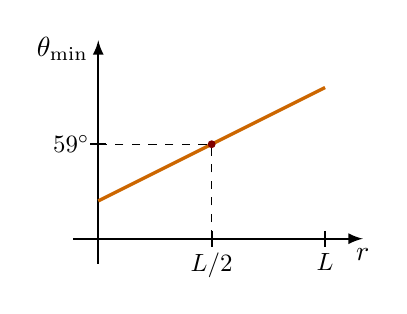
\begin{tikzpicture}
  \message{Minimum angle vs. r^^J}
  \def\xmax{3.2}
  \def\ymax{2.4}
  \coordinate (O) at (0,0);
  \coordinate (B) at (0.45*\xmax,0.5*\ymax);
  \coordinate (Bx) at (0.45*\xmax,0);
  \coordinate (By) at (0,0.5*\ymax);
  \draw[->,thick] (0,-0.1*\xmax) -- (0,1.05*\ymax) node[below=3,left] {$\theta_\text{min}$};
  \draw[->,thick] (-0.1*\xmax,0) -- (1.05*\xmax,0) node[below] {$r$}; %\mu_\mathrm{s}
  \draw[very thick,orange!80!black] (0,0.2*\ymax) -- (0.9*\xmax,0.8*\ymax);
  \draw[dashed] (Bx) |- (By);
  \tick{Bx}{90} node[below=-1,scale=0.9] {$L/2$};
  \tick{0.9*\xmax,0}{90} node[below=-1,scale=0.9] {$L$};
  \tick{By}{0} node[right=3,left=0,scale=0.9] {$\SI{59}{\degree}$};
  \fill[red!50!black] (B) circle(0.05);
\end{tikzpicture}


\end{document}
